\subsection{研究内容}\label{ch2content}

本项目面向深度学习模型测试的实际需求,突破人工智能安全的前沿挑战,针对深度学习测
试存在的伸缩性差、测试结果可解释性匮乏、测试数据标注成本高等问题,以知识萃取和可
解释机器学习为基础手段,研究基于决策行为模拟的黑盒测试、基于层次语义理解的白盒测
试和融合反馈偏置的自适应测试集生成,突破黑盒模型决策路径模拟、深度学习模型层次语
义理解和可解释测试集生成等关键技术,建立全生命周期的可解释测试方法,并在自动驾
驶、人脸识别等实际应用场景检验本项目研究成果。


项目研究工作从黑盒测试、白盒测试和测试集生成三个方面展开,本项目的挑战、科学问题
和研究内容关系如图~\ref{fig:ch2:rc}所示。各部分研究内容具体介绍如下:

\begin{figure}[htp]
    \begin{small}
        \begin{center}
            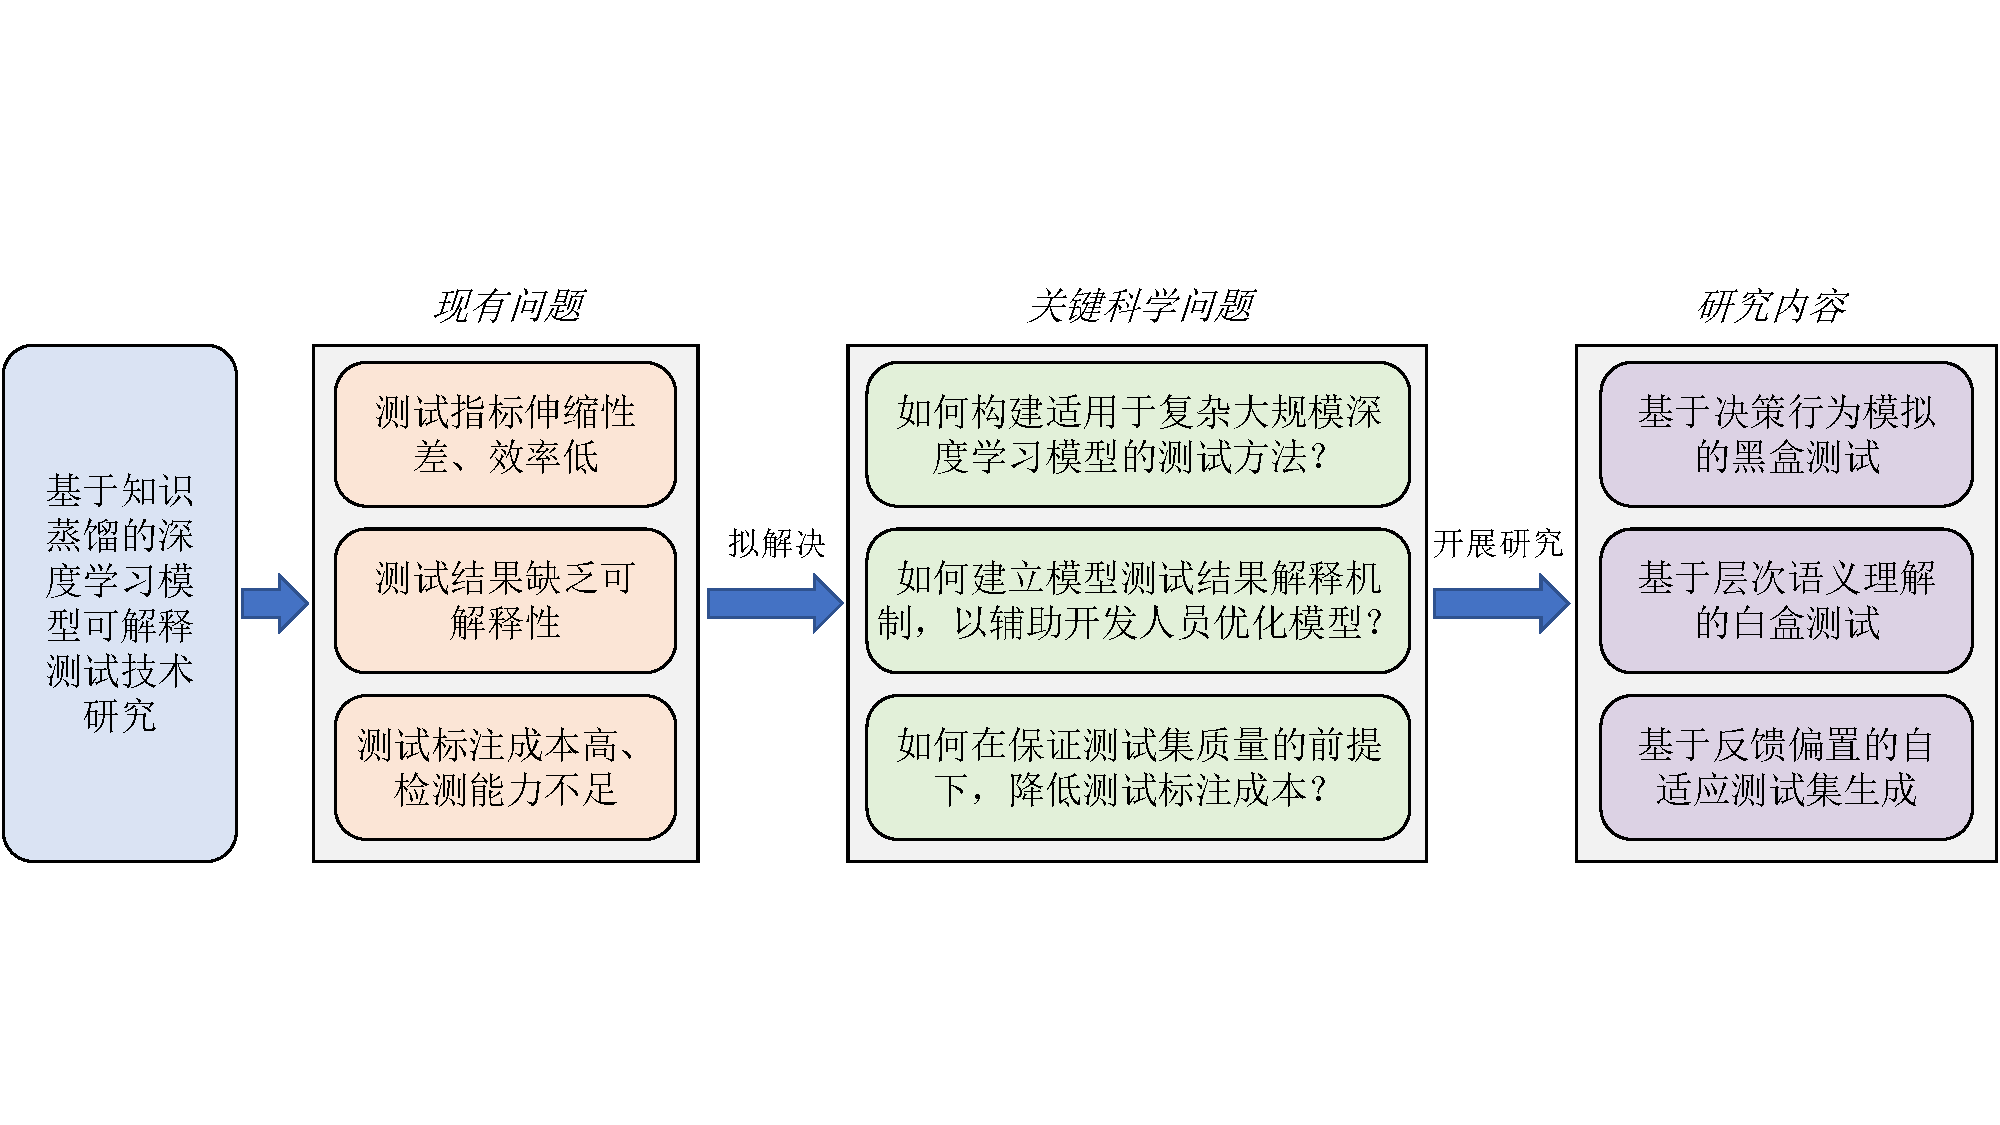
\includegraphics[width=0.95\textwidth]{ch2_framework.pdf}
        \end{center}
        \caption{挑战、科学问题和研究内容关系图}
        \label{fig:ch2:rc}
    \end{small}
\end{figure}

\subsubsection{基于决策行为模拟的黑盒测试}

借鉴传统软件的路径覆盖测试方法,许多研究提出针对深度学习模型的覆盖性测试方法(参
见\ref{relatedwork} 国内外研究现状及发展动态分析),这些测试覆盖指标和方法主要是
针对白盒的场景,即测试者掌握所有的训练数据和整个深度学习模型,\textbf{但在许多场
景中,测试者无法访问训练数据和模型内部结构,但仍需要对模型的泛化能力进行测试,即
黑盒测试,如深度学习模型是某个公司私有的或者由第三方机构提供,他们只提供了接口或
者打包的可执行程序。}因此,本项目面向黑盒测试场景,研究基于决策行为模拟的黑盒测
试方法。

以分类模型为例,给定一个黑盒深度学习模型$\mathcal M$和测试数据集$\mathcal
D_{\text{test}}=\{x^{(i)},y^{(i)}\}$,测试者可以得到模型针对每个输入
$x^{(i)}$(input)的输出$\hat{y}^{(i)}$,通常是该输入属于各个类别的概率分布,除
此之外,测试者无法知道该模型的训练数据和内部结构。可见,深度学习模型黑盒测试面临
两个主要问题:
\begin{itemize}
    \item \textbf{如何建立模型有关的测试方法?}仅有的几个黑盒模型测试方法仅针对
    数据的多样性进行评估,无法准确反映模型的性能,也不能给模型改进提供有效建议。
    \item \textbf{如何掌握模型的决策机制?}黑盒测试中,测试者无法了解模型的结
    构,模型对测试用例的决策过程无法知晓。
\end{itemize}

\begin{figure}[htp]
    \begin{small}
        \begin{center}
            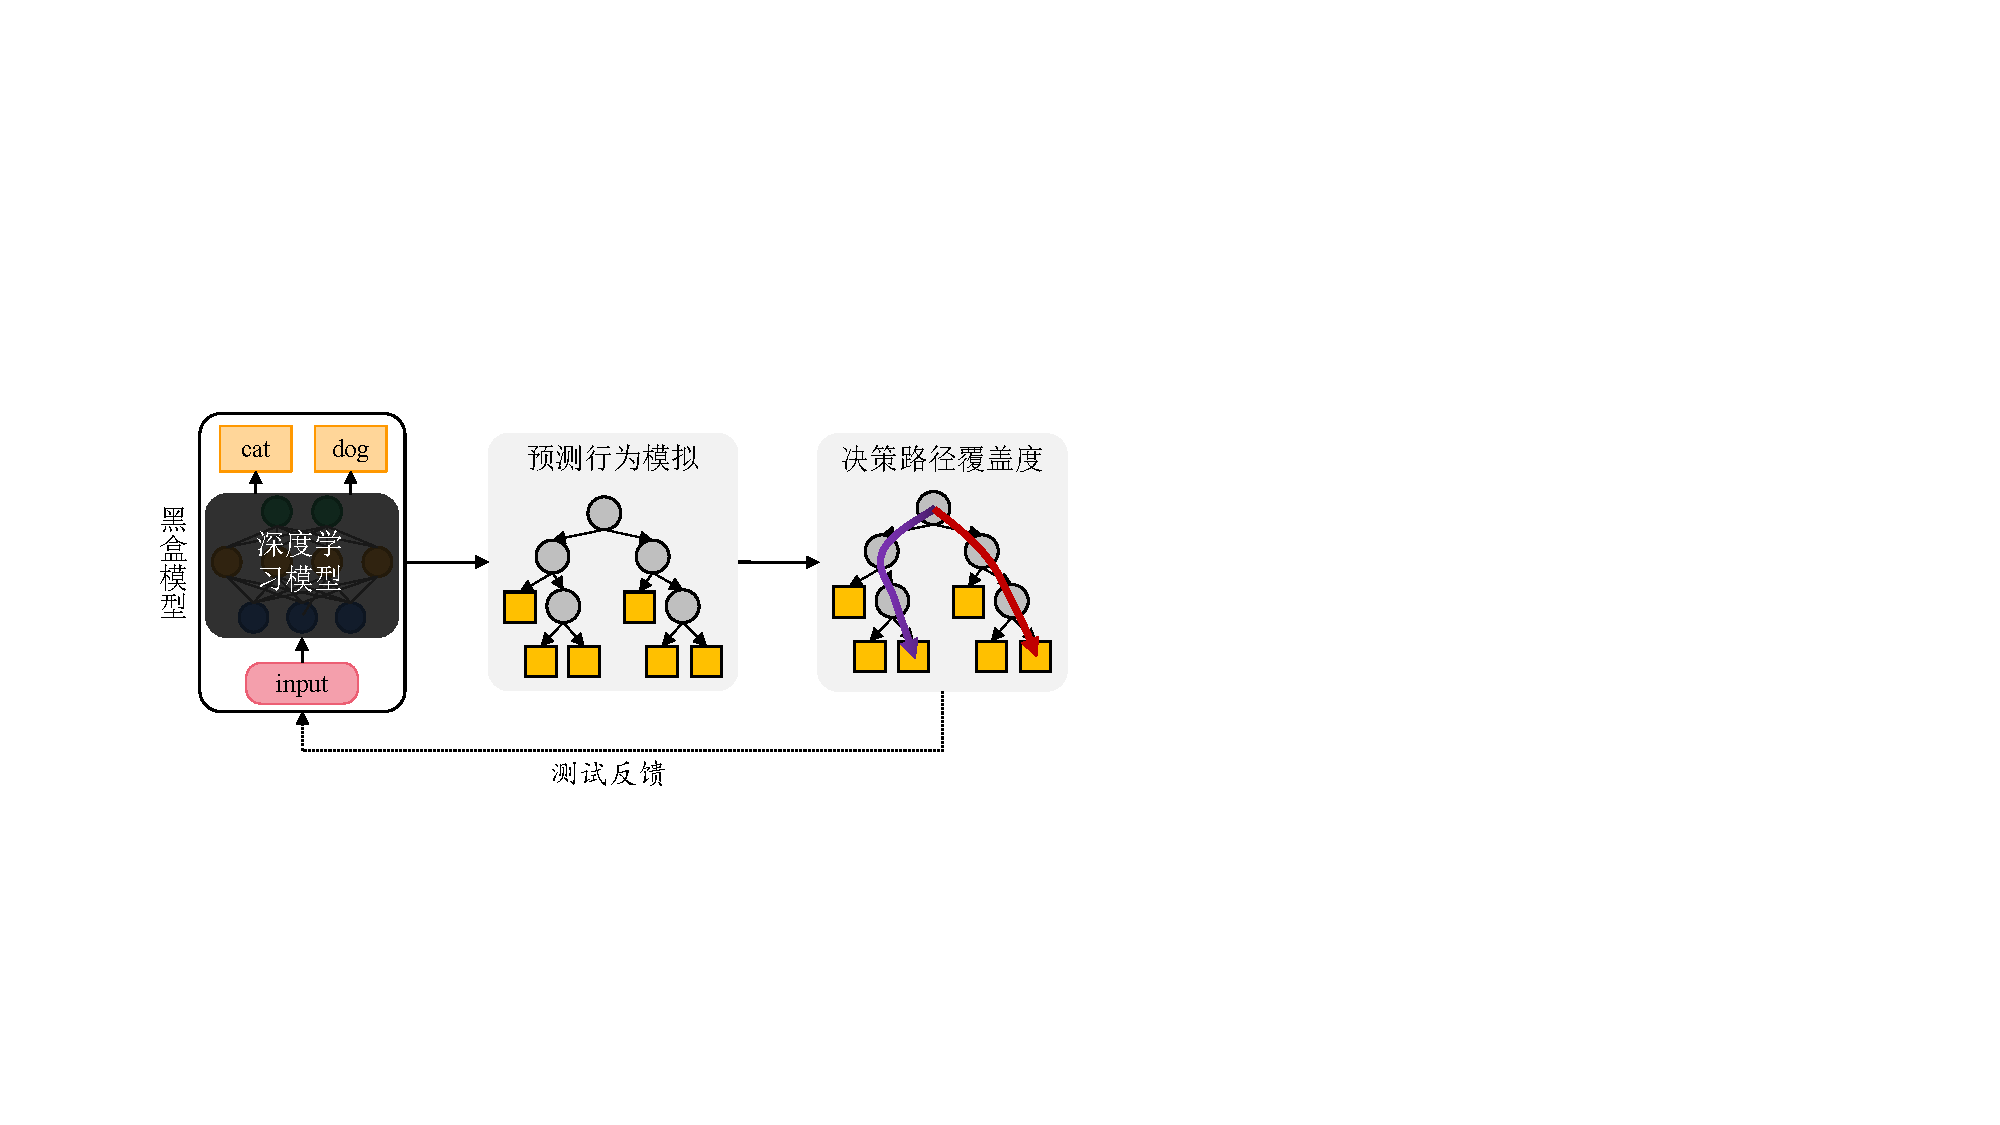
\includegraphics[width=0.75\textwidth]{ch2_2Btest.pdf}
        \end{center}
        \caption{基于决策行为模拟的黑盒测试研究内容}
        \label{fig:ch2:2Btest}
    \end{small}
\end{figure}
本项目深度学习模型黑盒测试的主要研究内容如\cref{fig:ch2:2Btest}所示,\textbf{本项目首先
研究针对黑盒模型的预测行为模拟方法,拟利用知识萃取的方法,通过建立副本模型
$\mathcal M^\prime$(如决策树)萃取黑盒模型$\mathcal M$的知识,模拟$\mathcal M$
的预测行为;然后,在副本模型的基础上,本项目拟建立基于决策路径覆盖度的测试方法,
通过覆盖度指标反映模型的决策机制和泛化能力。}

\subsubsection{基于层次语义理解的白盒测试}

除了黑盒测试的场景,白盒测试的需求也非常多,如企业自己开发的深度学习模型,在白盒
测试中,测试者可以访问模型的内部结构$\mathcal M(\bm W, \bm b)$和训练数据集
$\mathcal D_{train}=\{(x^{(i)}, y^{(i)}\})$。目前,针对深度学习模型的白盒测试方
法可扩展性和可解释性较差,无法应用于大规模深度学习模型,如
BERT~\cite{kenton2019bert},MAE~\cite{he2021masked}等,而且测试结果无法给模型训
练提供有效反馈,辅助模型优化。因此,\textbf{本项目提出针对白盒深度学习模型的层次
语义理解方法,并利用各层的决策语义训练一个副本模型中,保证副本模型的决策路径与原
白盒模型一致;然后围绕副本模型进行决策路径覆盖度测试,决策路径具有较强的可解释
性,可引导测试数据生成和模型优化。}

\begin{figure}[htp]
    \begin{small}
        \begin{center}
            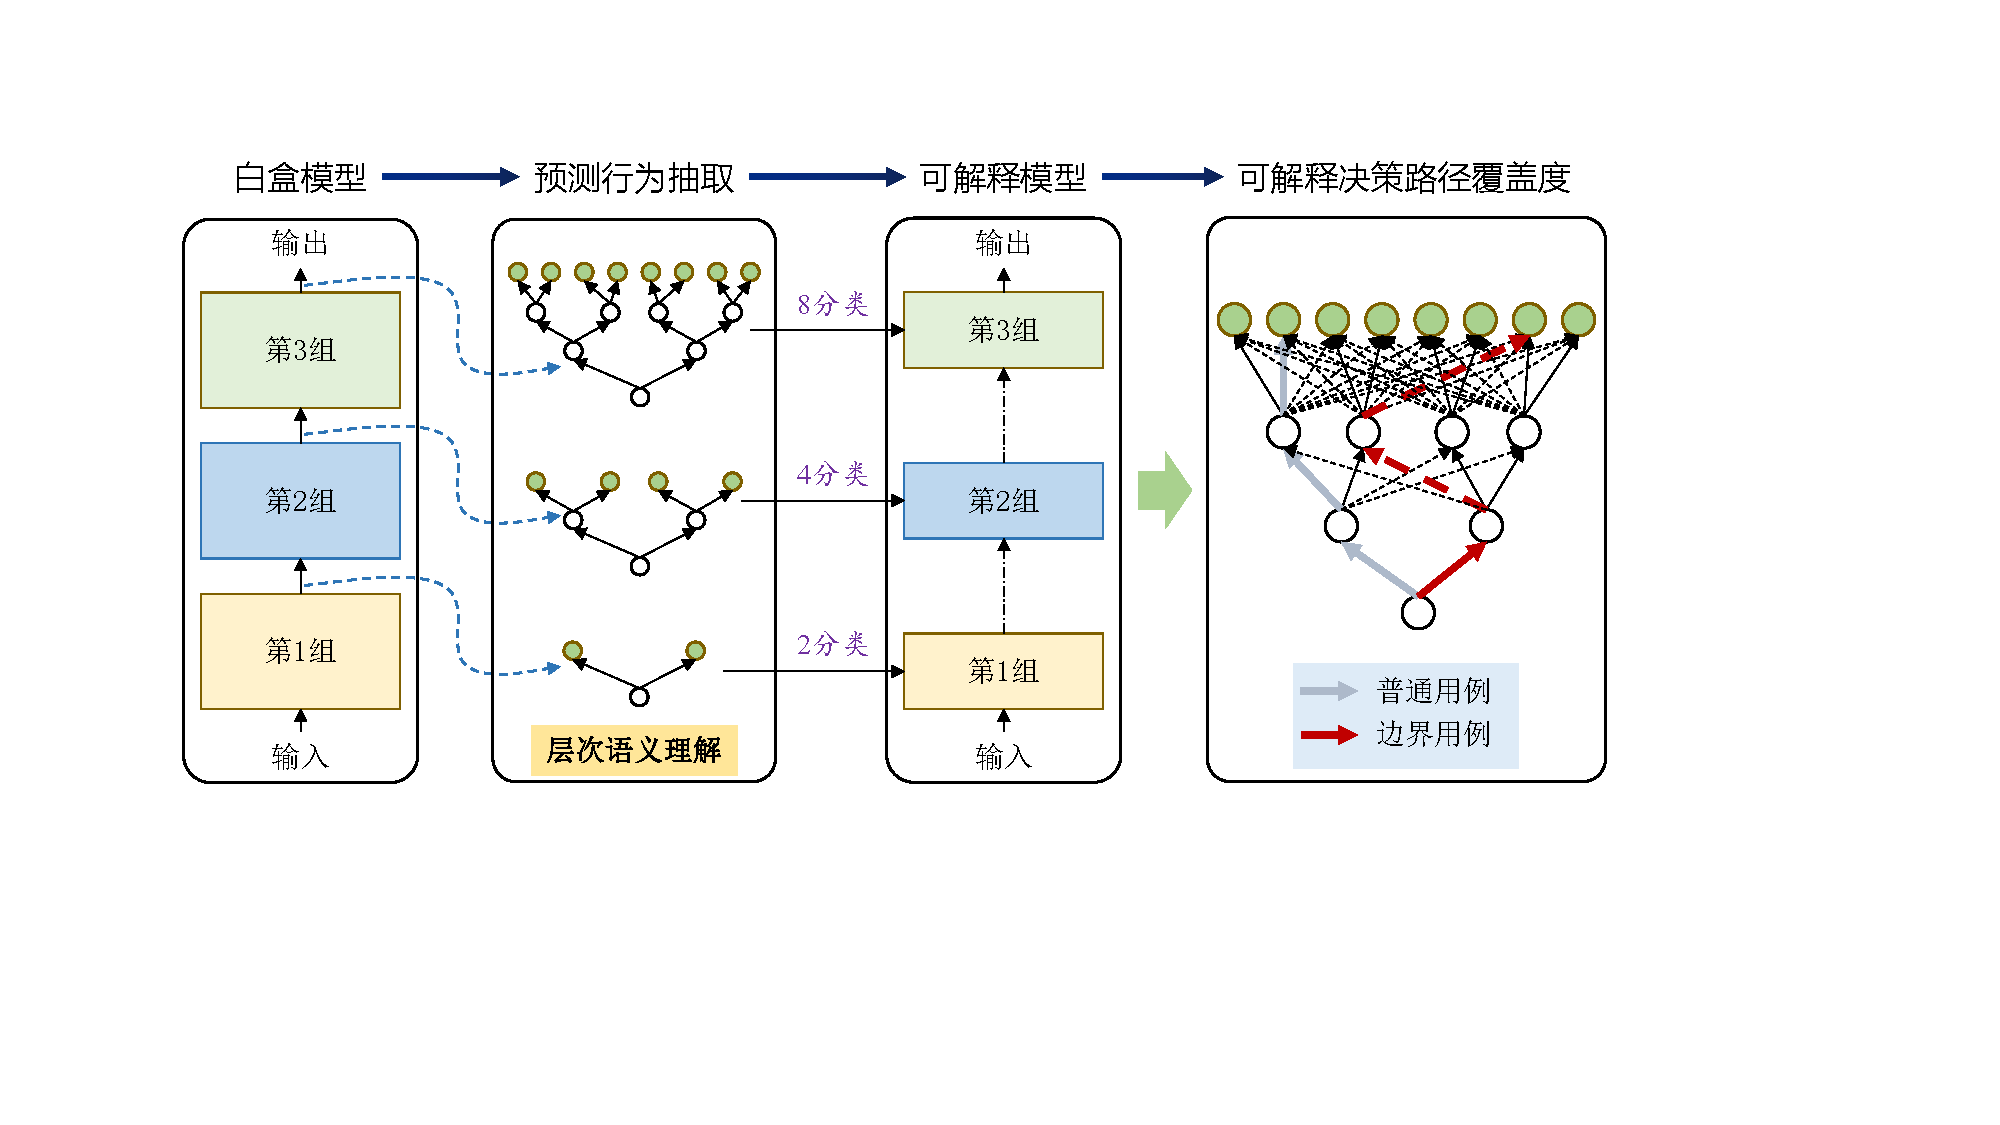
\includegraphics[width=0.9\textwidth]{ch2_WBtest.pdf}
        \end{center}
        \caption{基于层次语义理解的白盒测试研究内容}
        \label{fig:ch2:WBtest}
    \end{small}
\end{figure}

本项目基于层次语义理解的白盒测试研究内容如\cref{fig:ch2:WBtest}所示,在白盒测试
的场景下,本项目首先研究如何从深度学习模型中抽取出各层(layer)的决策语义信息,
研究表明,深度学习模型对输入的决策是由粗粒度到细粒度的。\cref{fig:ch2:WBtest}举
例说明了从3组神经网络层的输出抽取各组网络的预测行为,例如:输入一个猫的图片,第1
组神经网络判断该图片是否是动物,接着,第2组神经网络判断该图片是否是猫科动物,最
后,第3组神经网络将该图片分类为猫。\textbf{本项目拟研究如何实现层次语义理解,自
动地从深度学习模型中抽取出各层的决策语义}。

在层次语义理解的基础上,\textbf{本项目拟融合白盒模型的多层次决策语义训练一个副本
模型,使该副本模型的决策路径与原白盒模型一致,且具有良好的可解释性}。此外,知识
蒸馏得到的模型通常规模较小,和直接测试原白盒模型相比,测试副本模型可有效提高测试
效率。\textbf{在得到可解释的副本模型后,本项目拟研究并提出针对该可解释模型的决策
路径覆盖度,用于分析测试样本的多样性和充分性}。

\subsubsection{融合反馈偏置的自适应测试集生成}
深度学习模型的测试依赖于有标签的测试集,以判断模型预测结果是否符合预期,然而,测
试集的标签通常依赖于人工标注,成本较高,而测试集规模较大,难以标注并测试每个输入
数据。因此,{需要合理平衡测试集的规模和质量,在有限标注成本空间内选取根据测试目
标选取测试数据,生成规模可控制的高质量测试集}。\textbf{本项目拟提出一种基于决策
路径的自适应测试集生成方法,针对大规模无标注测试数据,融合反馈偏置和自适应测试,
筛选出具有不同检测能力的测试数据,生成规模可控的高效测试集。}

\begin{figure}[htp]
    \begin{small}
        \begin{center}
            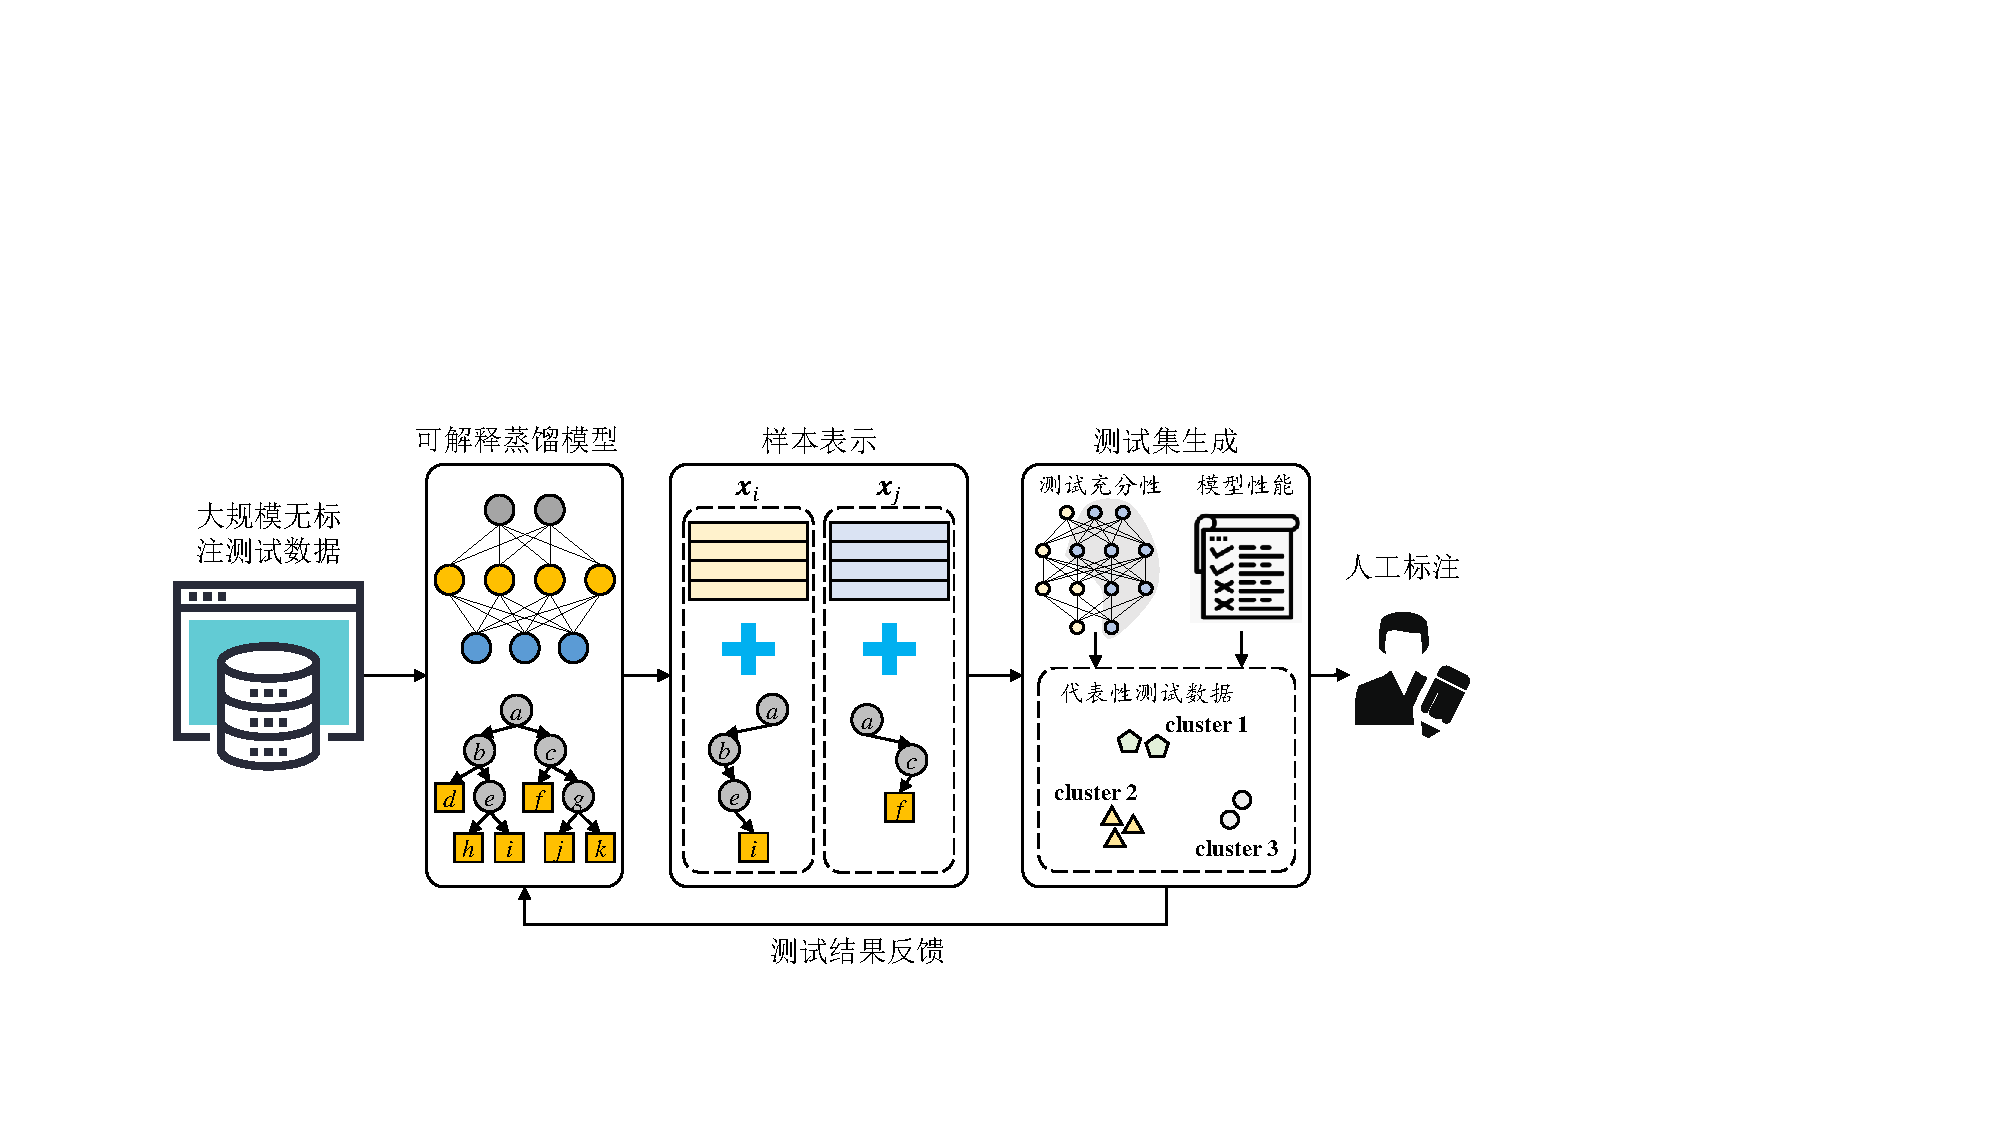
\includegraphics[width=0.95\textwidth]{ch2_TestSelection.pdf}
        \end{center}
        \caption{可解释预测模型研究内容}
        \label{fig:ch2:testselection}
    \end{small}
\end{figure}

如\cref{fig:ch2:testselection}所示,给定大规模无标注测试数据,{本项目选取两类测
试数据构建测试集:\textbf{一类是代表性数据},即能够模拟大规模无标注测试数据分布
的小规模测试子集,以达到高效度量模型性能的目的;\textbf{第二类是边界数据},融合
自适应测试和反馈偏置,找到可能导致模型错误行为的边界测试数据,以达到充分性测试的
目的}。针对第一个测试目标,本项目拟研究样例测试数据选取,结合决策路径和样本表
示,构建可解释的代表性测试集生成方法。针对第二个测试目标,本项目拟融合自适应测试
和反馈偏置,对已选取的测试数据进行标注并测试,并根据测试结果的反馈偏置,持续性筛
选未标注测试数据中的离群点和可能导致模型错误行为的边界数据。


%1.代表性数据筛选,能够用小规模测试数据模拟大规模无标注数据的决策路径分布,准确评估模型性能

%2.边界数据选取,对模型进行充分性测试,找到导致模型错误行为的测试数据标注

\subsection{研究目标}\label{ch2target}

本项目从深度学习模型部署的实际需求和人工智能软件安全性的前沿问题出发,针对深度学
习模型测试方法伸缩性差、缺乏可解释性和测试数据标注成本高等问题,分别建立基于决策
路径的黑盒测试和白盒测试方法,在此基础上构建融合反馈偏置的自适应测试集生成方法,
形成一套从测试指标、测试用例生成到测试反馈的深度学习可解释测试解决方案,并在自动
驾驶、人脸识别等实际应用中检验研究成果的效果。

具体研究目标包括:

\textbf{在技术方面},本项目拟在以下三方面实现技术突破: (a) 提出基于决策行为模拟
的黑盒测试方法,利用知识蒸馏技术,训练副本模型,模拟黑盒模型的预测行为,实现伸缩
性强、可解释性的黑盒测试;(b) 提出基于层次语义理解理解的白盒测试方法,抽取模型的
中间表示和决策路径,训练副本模型,实现伸缩性强、可解释的白盒测试;(c) 提出融合反
馈偏置的自适应测试集生成方法,针对测试目标,结合测试执行反馈,选取与大规模无标注
测试数据具有近似决策路径分布的代表性数据。

\textbf{在成果形式方面},本项目力争在CCF-A类推荐期刊/会议或其他SCI期刊上发表高水
平论文3-6篇;申请专利2项;并开源相关研究工作,供用户下载,并提供说明和使用文档。

\textbf{在人才培养方面},通过本项目研究,培养深度学习测试、人工智能安全等前沿领
域的青年人才,拟培养研究生2-3人。

\subsection{拟解决的关键科学问题}

基于上述研究目标和研究内容,本项目拟在以下几个关键理论和技术问题上有所突破:

\subsubsection{在黑盒场景下,仅根据模型输入输出,模拟构建黑盒模型的决策路径}

在黑盒测试中,测试者无法了解待测模型的内部结构和训练数据集,仅能得到测试输入输
出,因此无法知晓模型对输入样本是如何决策判断的。现有测试覆盖指标主要基于神经网络
结构的覆盖,仅有黑盒测试研究局限于与模型无关的测试数据多样性的评估,尚未建立模型
有关的黑盒测试方法,无法提供针对特定模型的测试逻辑。因此,在黑盒测试中,如何通过
输入输出模拟模型的决策路径,建立基于决策路径的测试覆盖度指标,以实现可解释黑盒测
试是本项目拟解决的一个关键科学问题。


\subsubsection{在白盒场景下,分层抽象模型内在决策路径,建立基于决策路径的测试覆盖指标}

在白盒测试中,测试者可以得到模型的内部结构和训练数据集,但是深度学习模型的可解释
性差,难以知晓模型对于特定样本是如何决策判断的。另一方面,现有深度学习测试的研究
主要围绕神经元取值和覆盖度进行分析,不仅计算复杂度高,难以应用于大模型,而且缺乏
语义可解释性,相应的测试报告无法给模型开发人员提供有效指导。因此,在白盒测试中,
如何分层抽象深度学习模型内在的决策路径,以实现基于决策路径的可解释测试是本项目拟
解决的另一个关键科学问题。

\subsubsection{在决策路径覆盖引导下,融合反馈偏置筛选规模可控的测试数据评估模型性能}

深度学习模型测试依赖于数据标注,实际应用中,需要合理平衡测试集的规模和质量,在有
限标注成本空间内选取对样本空间最具代表性的测试数据。在本项目黑盒和白盒决策路径覆
盖测试的基础上,已选择的测试数据执行结果可为后续测试数据选择提供模型正确性反馈和
路径覆盖反馈,指导后续测试数据筛选方式,因此,如何对这种反馈偏置进行形式化建模,
将其用于代表性测试用例的持续筛选中,并适应不同的测试目标,也是本项目拟解决的关键
科学问题问题之一。